%%%%%%%%%%%%%%%%%%%%%%%%%%%%%%%%%%%%%%%%%%%%%%%%%%%%%%%%%%%%%%%%%%%%%
%  Emotion-Aware Image Caption Generation -- Final Presentation
%  Machine Learning Sessional  |  TeamML Newbies
%  Template: Madrid Beamer theme (following proposal.tex style)
%%%%%%%%%%%%%%%%%%%%%%%%%%%%%%%%%%%%%%%%%%%%%%%%%%%%%%%%%%%%%%%%%%%%%

\documentclass{beamer}
\usetheme{Madrid}
\usecolortheme{whale}

\usepackage{graphicx}
\usepackage{tikz}
\usetikzlibrary{shapes,arrows,positioning,calc,fit,backgrounds,shadows}
\usepackage{hyperref}
\usepackage{amsmath}
\usepackage{amssymb}
\usepackage{booktabs}
\usepackage{colortbl}
\usepackage{pgfplots}
\pgfplotsset{compat=1.18}

%% ── Colour palette ──────────────────────────────────────────────────
\definecolor{vitblue}{RGB}{30,80,160}
\definecolor{gptpurple}{RGB}{110,40,160}
\definecolor{deepgreen}{RGB}{20,130,60}
\definecolor{emotionorange}{RGB}{210,100,10}
\definecolor{lightgray}{RGB}{240,240,240}

%% ── Title / Author info ─────────────────────────────────────────────
\title{Emotion-Aware Image Caption Generator}
\subtitle{Machine Learning Sessional -- Final Presentation}
\author{}
\newcommand{\authorinfo}{
    \begin{tabular}{rl}
    \textbf{Team:} & TeamML\_Newbies \\[0.3em]
    \end{tabular}

    \vspace{0.25cm}

    \begin{tabular}{rl}
    Anuron Maitro          & (2105037) \\
    Md. Asif Ali           & (2105038) \\
    Himadri Gobinda Biswas & (2105047)
    \end{tabular}
}
\date{}

%%%%%%%%%%%%%%%%%%%%%%%%%%%%%%%%%%%%%%%%%%%%%%%%%%%%%%%%%%%%%%%%%%%%
\begin{document}
%%%%%%%%%%%%%%%%%%%%%%%%%%%%%%%%%%%%%%%%%%%%%%%%%%%%%%%%%%%%%%%%%%%%

%% ═══════════════════════════════════════════════════════════════════
%% SLIDE 1 — Title
%% ═══════════════════════════════════════════════════════════════════
\begin{frame}
    \titlepage
    \vspace{-0.8cm}
    \begin{center}
        \authorinfo
    \end{center}
\end{frame}

%% ═══════════════════════════════════════════════════════════════════
%% SLIDE 2 — Introduction & Motivation
%% ═══════════════════════════════════════════════════════════════════
\begin{frame}{Introduction \& Motivation}

    \textbf{What is Image Captioning?}
    \begin{itemize}
        \item Automatically generating natural-language descriptions for images
        \item Traditional systems describe \textit{what} is in the image
    \end{itemize}

    \vspace{0.3cm}
    \textbf{The Gap — What is Missing?}
    \begin{itemize}
        \item A photo of a person on a beach $\Rightarrow$
              \textcolor{gray}{``A person standing on a beach''}
        \item But \textit{how does the person feel?} — Machines ignore this
    \end{itemize}

    \vspace{0.3cm}
    \textbf{Our Motivation:}
    \begin{itemize}
        \item \textbf{Accessibility:} Richer descriptions for visually impaired users
        \item \textbf{Human-AI Interaction:} More empathetic, contextual AI
        \item \textbf{Social Media / Healthcare:} Emotional context adds value
    \end{itemize}

    \vspace{0.2cm}
    \begin{block}{Our Innovation}
        \centering
        \textbf{Standard Caption} $\xrightarrow{\text{+Emotion}}$
        \textbf{Emotion-Aware Caption}\\[0.1em]
        \small ``A person on a road'' $\rightarrow$
        ``A \textit{joyful} person on a road''
    \end{block}
\end{frame}

%% ═══════════════════════════════════════════════════════════════════
%% SLIDE 3 — Problem Statement & Approach
%% ═══════════════════════════════════════════════════════════════════
\begin{frame}{Problem Statement \& Our Approach}

    \textbf{Problem:}\\
    \textit{How can we generate captions that describe \textbf{both} the visual
    content \textbf{and} the emotional state of people in the image?}

    \vspace{0.4cm}
    \textbf{Three Sub-Challenges:}
    \begin{enumerate}
        \item \textbf{Base Caption Generation} : accurate visual description
        \item \textbf{Emotion Detection} : detect facial emotion reliably
        \item \textbf{Natural Language Integration} : merge them grammatically
    \end{enumerate}

    \vspace{0.4cm}
    \textbf{Our Three-Component Solution:}
    \begin{itemize}
        \item \textcolor{vitblue}{\textbf{ViT + GPT-2}} — for high-quality base captions
        \item \textcolor{emotionorange}{\textbf{DeepFace}} — for 7-category emotion recognition
        \item \textcolor{deepgreen}{\textbf{NLTK POS Tagger}} — for grammatical emotion insertion
    \end{itemize}

\end{frame}

%% ═══════════════════════════════════════════════════════════════════
%% SLIDE 4a — Complete System Pipeline (Part 1: Stages 1 & 2)
%% ═══════════════════════════════════════════════════════════════════
\begin{frame}{Complete System Pipeline (1/2)}

\begin{center}
\scalebox{0.62}{%
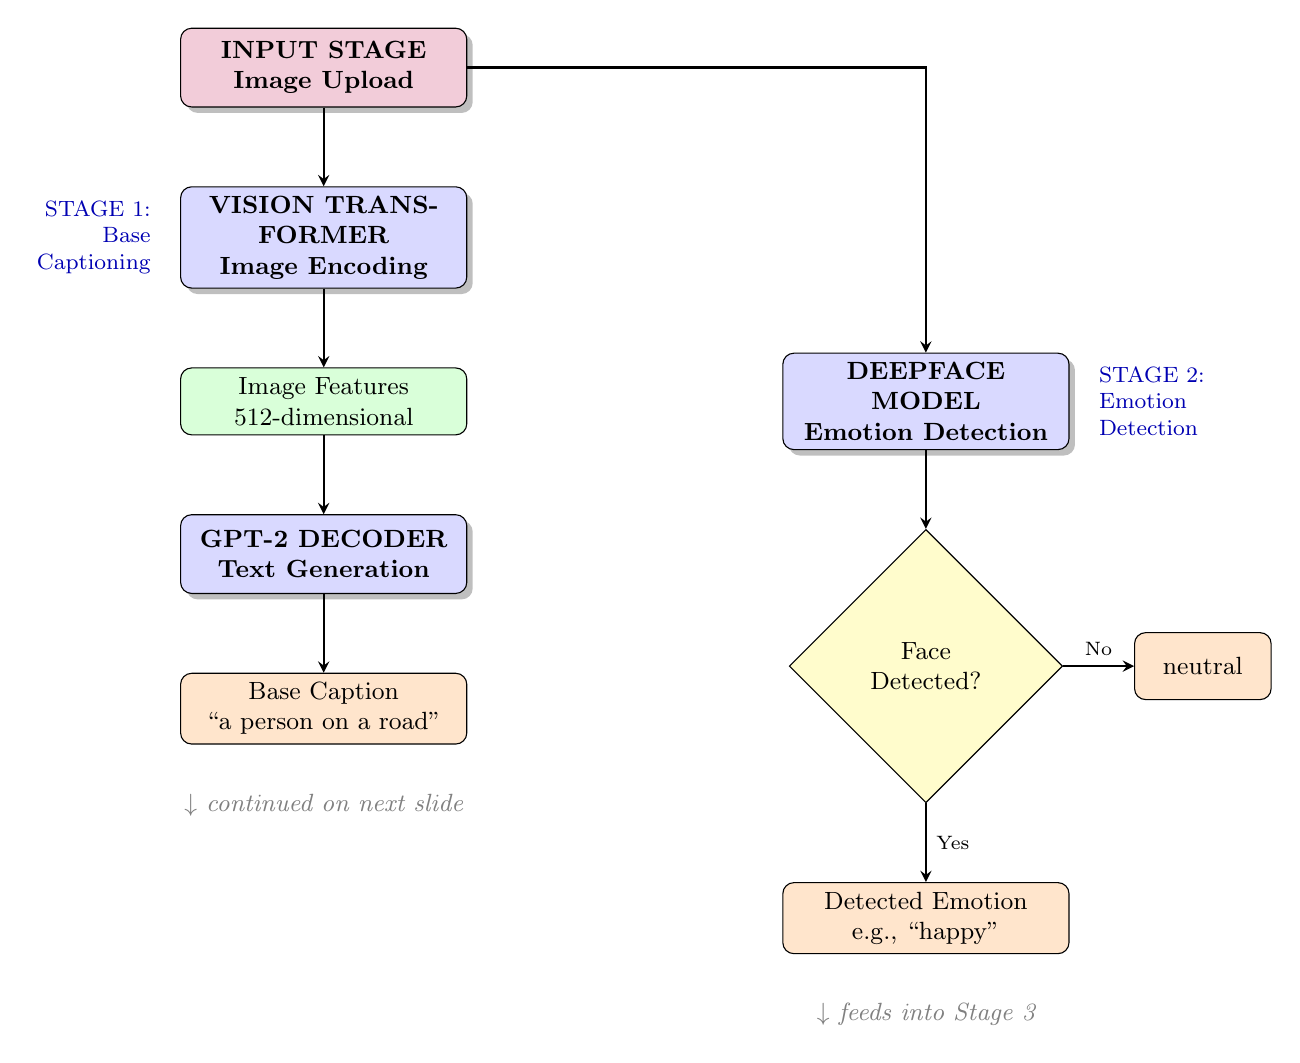
\begin{tikzpicture}[
    node distance=1.0cm and 1.4cm,
    stage/.style={rectangle, draw, fill=blue!15, text width=3.4cm, text centered,
                  rounded corners, minimum height=1.0cm, drop shadow, font=\small\bfseries},
    process/.style={rectangle, draw, fill=green!15, text width=3.4cm, text centered,
                    rounded corners, minimum height=0.85cm, font=\small},
    output/.style={rectangle, draw, fill=orange!20, text width=3.4cm, text centered,
                   rounded corners, minimum height=0.85cm, font=\small},
    decision/.style={diamond, draw, fill=yellow!20, text width=2.4cm, text centered,
                     minimum height=1.0cm, font=\small},
    arrow/.style={->, >=stealth, thick},
    lbl/.style={font=\footnotesize, text=blue!70!black}
]

%% ── Left branch: Stage 1 ─────────────────────────────────────────
\node[stage, fill=purple!20] (input)  {INPUT STAGE\\Image Upload};
\node[stage,  below=of input]  (vit)   {VISION TRANSFORMER\\Image Encoding};
\node[process, below=of vit]   (vitout){Image Features\\512-dimensional};
\node[stage,  below=of vitout] (gpt)   {GPT-2 DECODER\\Text Generation};
\node[output, below=of gpt]    (basecap){Base Caption\\``a person on a road''};

%% ── Right branch: Stage 2 ────────────────────────────────────────
\node[stage,  right=4.0cm of vitout] (deepface){DEEPFACE MODEL\\Emotion Detection};
\node[decision, below=of deepface]   (detect)  {Face\\Detected?};
\node[output,   below=of detect]     (emotion) {Detected Emotion\\e.g., ``happy''};
\node[output,   right=0.9cm of detect, text width=1.5cm] (noemot) {neutral};

%% ── Arrows: left branch ──────────────────────────────────────────
\draw[arrow] (input)  -- (vit);
\draw[arrow] (vit)    -- (vitout);
\draw[arrow] (vitout) -- (gpt);
\draw[arrow] (gpt)    -- (basecap);

%% ── Arrows: right branch ─────────────────────────────────────────
\draw[arrow] (input.east)  -| (deepface.north);
\draw[arrow] (deepface)    -- (detect);
\draw[arrow] (detect) -- node[right,font=\scriptsize]{Yes} (emotion);
\draw[arrow] (detect) -- node[above,font=\scriptsize]{No}  (noemot);

%% ── Stage labels ─────────────────────────────────────────────────
\node[lbl, left=0.25cm of vit,      align=right] {STAGE 1:\\Base\\Captioning};
\node[lbl, right=0.25cm of deepface, align=left] {STAGE 2:\\Emotion\\Detection};

%% ── Continuation note ────────────────────────────────────────────
\node[lbl, below=0.5cm of basecap, align=center,
      font=\small\itshape, text=gray]
    {$\downarrow$ continued on next slide};
\node[lbl, below=0.5cm of emotion, align=center,
      font=\small\itshape, text=gray]
    {$\downarrow$ feeds into Stage 3};

\end{tikzpicture}
}
\end{center}
\end{frame}

%% ═══════════════════════════════════════════════════════════════════
%% SLIDE 4b — Complete System Pipeline (Part 2: Stage 3 + Output)
%% ═══════════════════════════════════════════════════════════════════
\begin{frame}{Complete System Pipeline (2/2)}

\begin{center}
\scalebox{0.65}{%
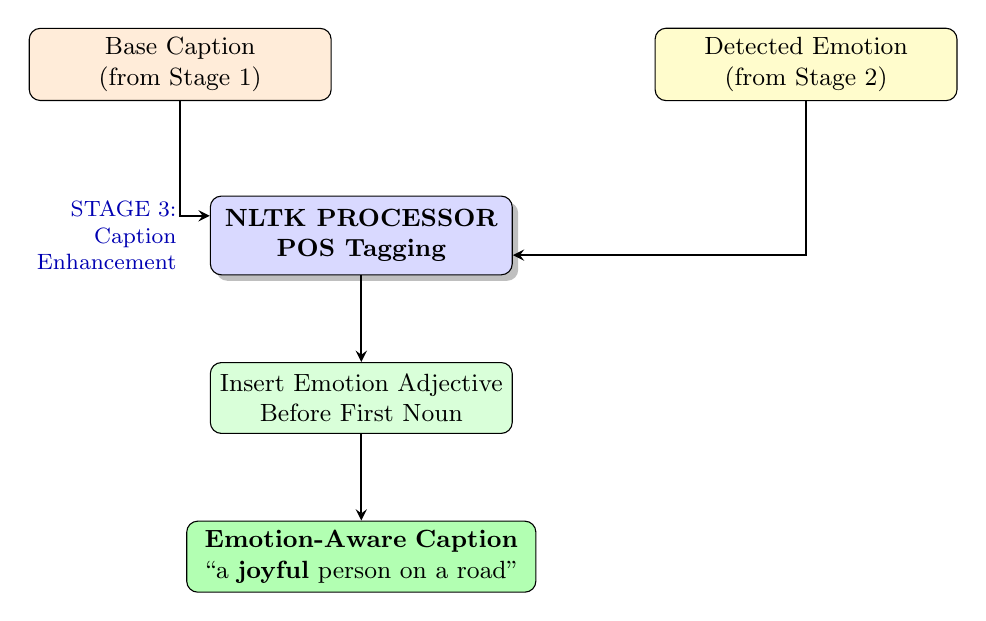
\begin{tikzpicture}[
    node distance=1.1cm and 1.5cm,
    stage/.style={rectangle, draw, fill=blue!15, text width=3.6cm, text centered,
                  rounded corners, minimum height=1.0cm, drop shadow, font=\small\bfseries},
    process/.style={rectangle, draw, fill=green!15, text width=3.6cm, text centered,
                    rounded corners, minimum height=0.9cm, font=\small},
    output/.style={rectangle, draw, fill=orange!20, text width=3.6cm, text centered,
                   rounded corners, minimum height=0.9cm, font=\small},
    arrow/.style={->, >=stealth, thick},
    lbl/.style={font=\footnotesize, text=blue!70!black}
]

%% ── Incoming from Stage 1 & 2 ────────────────────────────────────
\node[output, fill=orange!15, xshift=-0.6cm] (basein) {Base Caption\\(from Stage 1)};
\node[output, right=4.1cm of basein, fill=yellow!20] (emoin)
    {Detected Emotion\\(from Stage 2)};

%% ── Stage 3 ──────────────────────────────────────────────────────
\node[stage, below=1.2cm of basein, xshift=2.3cm] (nltk)
    {NLTK PROCESSOR\\POS Tagging};
\node[process, below=of nltk] (insert)
    {Insert Emotion Adjective\\Before First Noun};
\node[output,  below=of insert, fill=green!30, text width=4.2cm] (final)
    {\textbf{Emotion-Aware Caption}\\``a \textbf{joyful} person on a road''};

%% ── Arrows ───────────────────────────────────────────────────────
\draw[arrow] (basein.south)  |- ([yshift= 0.25cm]nltk.west);
\draw[arrow] (emoin.south)   |- ([yshift=-0.25cm]nltk.east);
\draw[arrow] (nltk)   -- (insert);
\draw[arrow] (insert) -- (final);

%% ── Stage label ──────────────────────────────────────────────────
\node[lbl, left=0.3cm of nltk, align=right] {STAGE 3:\\Caption\\Enhancement};

\end{tikzpicture}
}
\end{center}
\end{frame}

%% ═══════════════════════════════════════════════════════════════════
%% SLIDE 5a — ViT Encoder Architecture: Diagram Only
%% ═══════════════════════════════════════════════════════════════════
\begin{frame}{Base Captioning: Vision Transformer Encoder (1/2)}

%% Scale 0.53 maps the ~12cm-tall report diagram to ~6.4cm, fitting the Beamer content area.
\begin{center}
\scalebox{0.45}{%
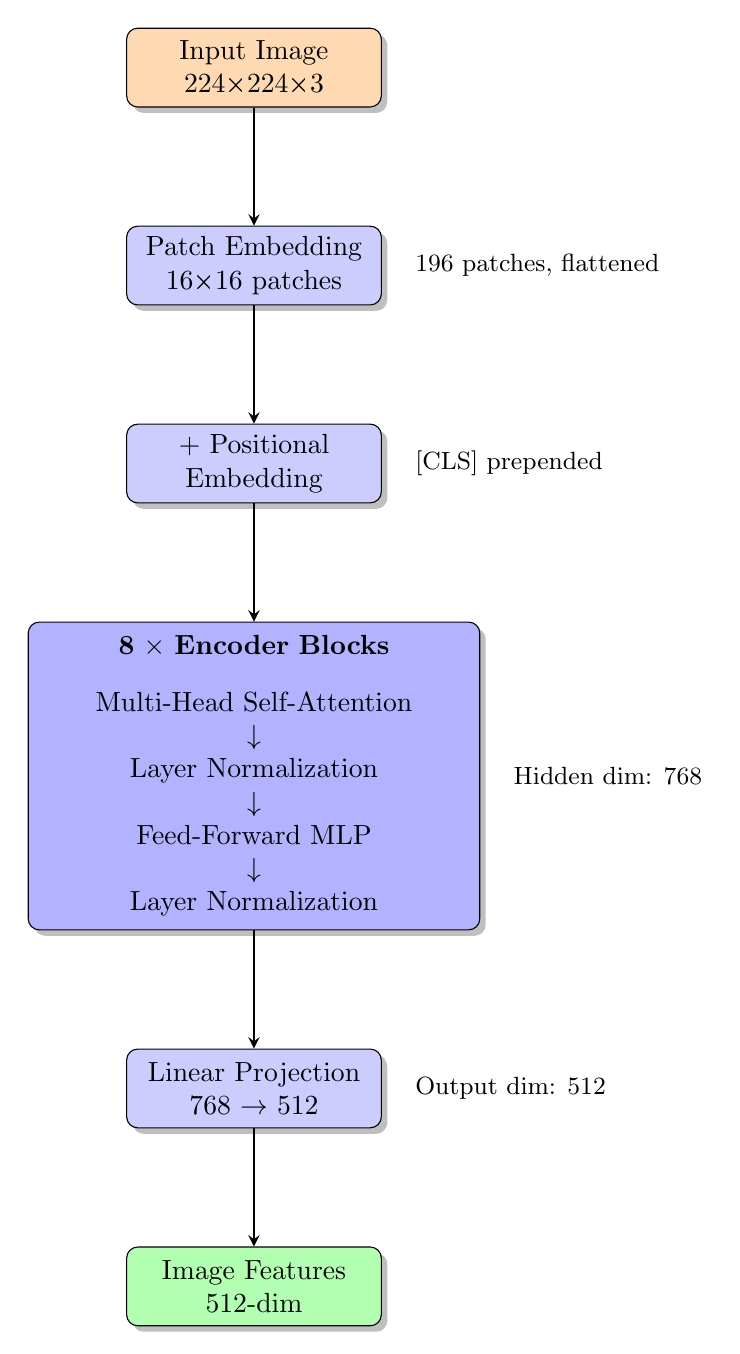
\begin{tikzpicture}[
    node distance=1.5cm and 2cm,
    block/.style={rectangle, draw, fill=blue!20, text width=3cm, text centered,
                  rounded corners, minimum height=1cm, drop shadow},
    arrow/.style={->, >=stealth, thick},
    lbl/.style={font=\small}
]
%% ── Nodes (exact order as report Figure 1) ───────────────────────
\node[block, fill=orange!30] (input) {Input Image\\224\texttimes224\texttimes3};

\node[block, below=of input] (patch) {Patch Embedding\\16\texttimes16 patches};
\node[lbl, right=0.3cm of patch] {196 patches, flattened};

\node[block, below=of patch] (pos)  {+ Positional\\Embedding};
\node[lbl, right=0.3cm of pos] {[CLS] prepended};

\node[block, below=of pos, minimum height=2.5cm, fill=blue!30, text width=5.5cm]
    (encoder) {
        \begin{tabular}{c}
        \textbf{8 $\times$ Encoder Blocks}\\[0.3cm]
        Multi-Head Self-Attention\\
        $\downarrow$\\
        Layer Normalization\\
        $\downarrow$\\
        Feed-Forward MLP\\
        $\downarrow$\\
        Layer Normalization
        \end{tabular}};
\node[lbl, right=0.3cm of encoder] {Hidden dim: 768};

\node[block, below=of encoder] (proj) {Linear Projection\\768 $\to$ 512};
\node[lbl, right=0.3cm of proj] {Output dim: 512};

\node[block, below=of proj, fill=green!30] (output) {Image Features\\512-dim};

%% ── Arrows ───────────────────────────────────────────────────────
\draw[arrow] (input)   -- (patch);
\draw[arrow] (patch)   -- (pos);
\draw[arrow] (pos)     -- (encoder);
\draw[arrow] (encoder) -- (proj);
\draw[arrow] (proj)    -- (output);
\end{tikzpicture}
}
\end{center}

\end{frame}


%% ═══════════════════════════════════════════════════════════════════
%% SLIDE 5b — ViT Encoder Architecture: Key Design Choices
%% ═══════════════════════════════════════════════════════════════════
\begin{frame}{Base Captioning: Vision Transformer Encoder (2/2)}

    \textbf{Key Design Choices:}\\[0.5em]
    \begin{itemize}
        \item Pre-trained \texttt{vit\_base\_patch16\_224} loaded from \texttt{timm} library
        \item Image divided into \textbf{196 patches} of $16\times16$ pixels each
        \item Each patch projected to \textbf{768-dim vector}
              \quad ($16^2 \times 3 = 768$)
        \item A \textbf{[CLS] token} is prepended; captures global image semantics
        \item \textbf{Learnable positional embeddings} added to all 197 tokens
        \item \textbf{8 Encoder Blocks}, each with \textbf{4 attention heads}, FFN (hidden 3072), LayerNorm \& Residual connections
        \item [CLS] token output (768-dim) passed through a \textbf{Linear Projection} layer to produce \textbf{512-dim image features}
    \end{itemize}

    \vspace{0.5cm}
    \begin{block}{Output}
        \centering
        A single \textbf{512-dim vector} representing the entire image.\\
        Used as cross-attention \textit{key} and \textit{value} in every GPT-2 decoder block.
    \end{block}

\end{frame}

%% ═══════════════════════════════════════════════════════════════════
%% SLIDE 6a — GPT-2 Decoder: Diagram Only
%% ═══════════════════════════════════════════════════════════════════
\begin{frame}{Base Captioning: GPT-2 Decoder (1/2)}

\begin{center}
\scalebox{0.43}{%
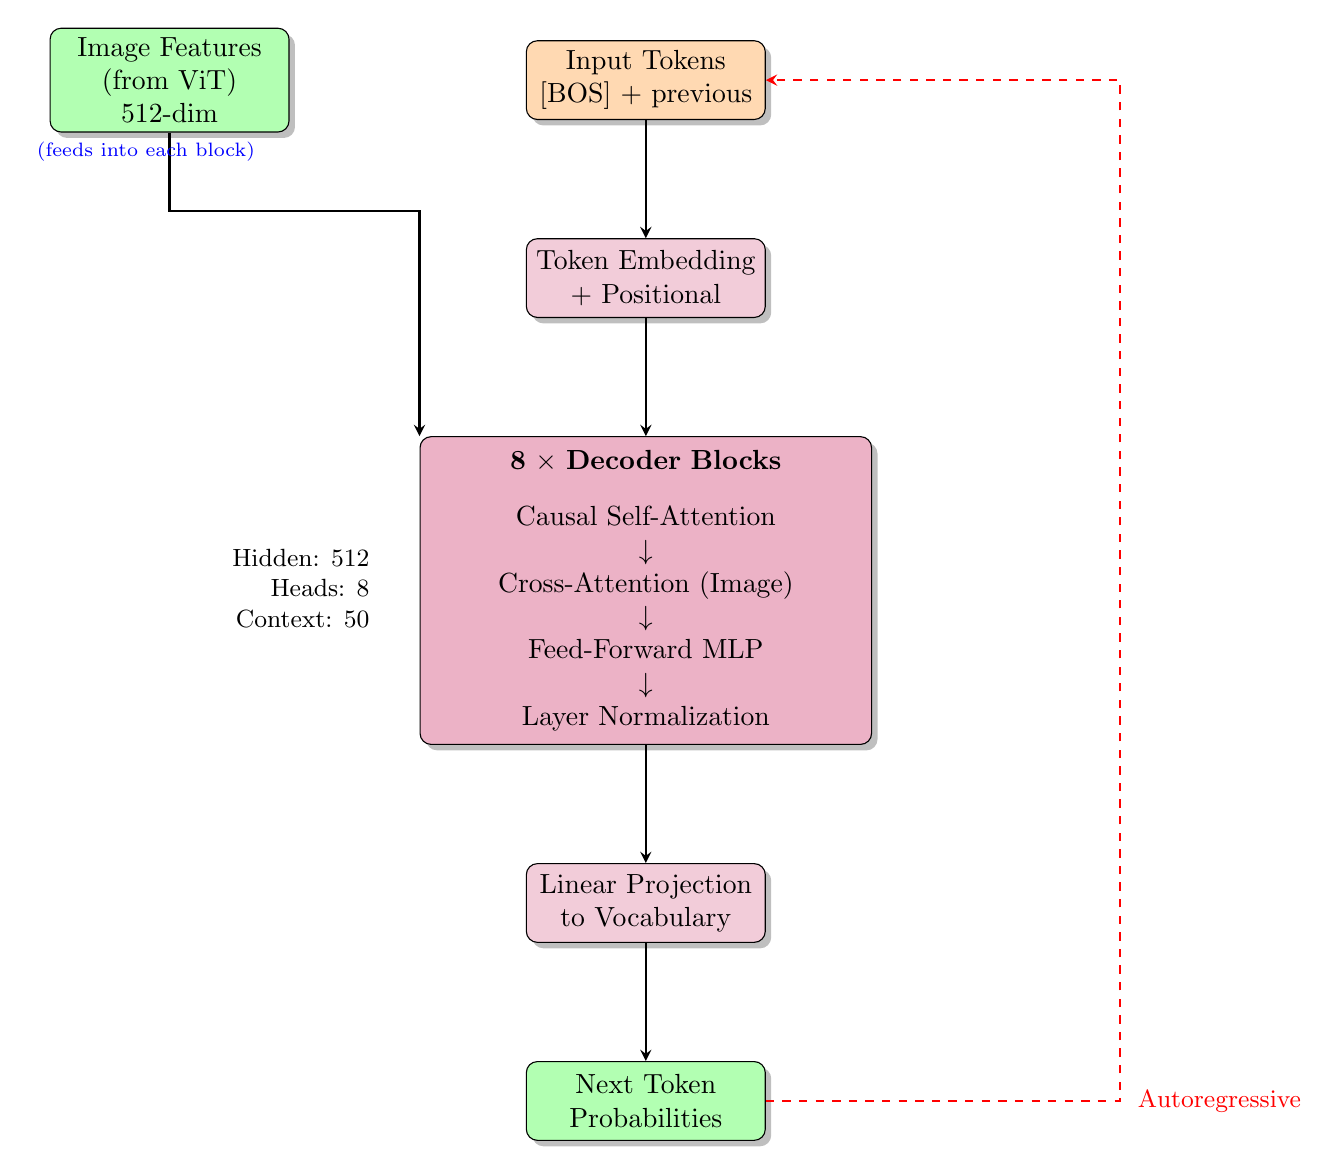
\begin{tikzpicture}[
    node distance=1.5cm and 1.5cm,
    block/.style={rectangle, draw, fill=purple!20, text width=2.8cm, text centered,
                  rounded corners, minimum height=1cm, drop shadow},
    arrow/.style={->, >=stealth, thick},
    lbl/.style={font=\small}
]
%% ── Nodes ───────────────────────────────────────────────────────
\node[block, fill=green!30]  (imgfeat) {Image Features\\(from ViT)\\512-dim};
\node[block, right=3cm of imgfeat, fill=orange!30]
                             (tokens)  {Input Tokens\\{[BOS]} + previous};

\node[block, below=of tokens]   (embed)  {Token Embedding\\+ Positional};

%% REMOVED: Cross-Attention block - not in actual code!

\node[block, below=1.5cm of embed, minimum height=3cm, fill=purple!30, text width=5.5cm]
    (decoder) {
        \begin{tabular}{c}
        \textbf{8 $\times$ Decoder Blocks}\\[0.3cm]
        Causal Self-Attention\\
        $\downarrow$\\
        Cross-Attention (Image)\\
        $\downarrow$\\
        Feed-Forward MLP\\
        $\downarrow$\\
        Layer Normalization
        \end{tabular}};

\node[block, below=of decoder] (proj)   {Linear Projection\\to Vocabulary};

\node[block, below=of proj, fill=green!30]
                             (output)  {Next Token\\Probabilities};

%% ── Forward arrows ───────────────────────────────────────────────
%% Image features go to decoder blocks (for cross-attention inside)
\draw[arrow] (imgfeat.south) -- ++(0,-1) -| (decoder.north west);

%% Tokens → Embedding → Decoder blocks DIRECTLY
\draw[arrow] (tokens)  -- (embed);
\draw[arrow] (embed)   -- (decoder);

\draw[arrow] (decoder) -- (proj);
\draw[arrow] (proj)    -- (output);

%% ── Autoregressive loop ─────────────────────────────────────────
\draw[arrow, dashed, red]
    (output.east) -- ++(4.5,0)
    |- (tokens.east);
\node[lbl, red, right=4.6cm of output] {Autoregressive};

%% ── Side annotation ──────────────────────────────────────────────
\node[lbl, left=0.3cm of decoder]
    {\begin{tabular}{r}Hidden: 512\\Heads: 8\\Context: 50\end{tabular}};

%% ── Optional: Add label showing image features feed into each block
\node[lbl, blue, left=0.3cm of imgfeat.south, anchor=north]
    {\scriptsize (feeds into each block)};
    
\end{tikzpicture}
}
\end{center}

\end{frame}

%% ═══════════════════════════════════════════════════════════════════
%% SLIDE 6b — GPT-2 Decoder: Key Design Choices
%% ═══════════════════════════════════════════════════════════════════
\begin{frame}{Base Captioning: GPT-2 Decoder (2/2)}

    \textbf{Key Design Choices:}\\[0.5em]
    \begin{itemize}
        \item GPT-2 tokenizer: 50,257 + 3 special tokens = 50,260 total
        \item \textbf{512-dim hidden state}, 8 attention heads per block
        \item \textbf{Causal Self-Attention} — masked so each token only attends to previous tokens (autoregressive property)
        \item \textbf{Cross-Attention} — every decoder block queries the 512-dim ViT image features, grounding text in visual content
        \item \textbf{Greedy Decoding} (argmax) at inference time
        \item Generation stops at \texttt{[EOS]} token or 50 tokens max
    \end{itemize}

    \vspace{0.4cm}
    \begin{columns}[T]
    \begin{column}{0.48\textwidth}
        \begin{block}{Special Tokens}
            \centering
            \texttt{[BOS]} \quad \texttt{[EOS]} \quad \texttt{[PAD]}\\
            \small Added to GPT-2 vocabulary during fine-tuning
        \end{block}
    \end{column}
    \begin{column}{0.50\textwidth}
        \begin{alertblock}{Autoregressive Loop}
            \small Generated token is fed back as next input. Continues until \texttt{[EOS]} or length 50.
        \end{alertblock}
    \end{column}
    \end{columns}

\end{frame}

%% ═══════════════════════════════════════════════════════════════════
%% SLIDE 7 — Emotion Detection (DeepFace) — fits in one page
%% ═══════════════════════════════════════════════════════════════════
\begin{frame}{Stage 2: Emotion Detection with DeepFace}

    \textbf{Why DeepFace?}
    \begin{itemize}
        \item State-of-the-art pre-trained facial emotion recognition
        \item No additional training required
        \item Used with \texttt{enforce\_detection=False} for robustness
        \item Returns dominant emotion from probability scores
    \end{itemize}

    \vspace{0.05cm}
    \textbf{7 Detected Emotion Categories:}\\[0.2em]
    \begin{center}
    \begin{tabular}{ccccccc}
    \textcolor{yellow!60!black}{\textbf{Happy}} &
    \textcolor{blue!60!black}{\textbf{Sad}} &
    \textcolor{red!70!black}{\textbf{Angry}} &
    \textcolor{orange!70!black}{\textbf{Surprise}} &
    \textcolor{purple!70!black}{\textbf{Fear}} &
    \textcolor{green!40!black}{\textbf{Disgust}} &
    \textcolor{gray!70!black}{\textbf{Neutral}}
    \end{tabular}
    \end{center}

    \vspace{0.05cm}
    \textbf{Processing Steps:}
    \begin{enumerate}
        \item Image temporarily saved as JPEG
        \item DeepFace analyzes facial expressions
        \item Dominant emotion extracted from result
        \item Falls back to \textit{neutral} if no face detected
    \end{enumerate}

    \vspace{0.2cm}
    \begin{alertblock}{Fallback Behaviour}
        If no face is detected (landscape or objects only), emotion defaults to \textbf{``neutral''} and the caption is enhanced with the adjective ``calm''.
    \end{alertblock}

\end{frame}

%% ═══════════════════════════════════════════════════════════════════
%% SLIDE 8 — NLTK Emotion Integration
%% ═══════════════════════════════════════════════════════════════════
\begin{frame}{Stage 3: NLTK-Based Grammatical Insertion}

\begin{columns}[T]
\begin{column}{0.48\textwidth}
    \textbf{Algorithm:}
    \begin{enumerate}
        \item Tokenize base caption
        \item POS-tag each token
        \item Find first \textbf{noun} (tag $\rightarrow$ \texttt{NN*})
        \item Insert emotion adjective \textit{before} that noun
        \item Reconstruct caption
    \end{enumerate}
    \vspace{0.3cm}
    \textbf{Example:}\\
    \small
    \textit{``a person standing on a road''}, Emotion: \textbf{happy}\\[0.2em]
    POS: \texttt{[DT,NN,VBG,IN,DT,NN]}\\
    First noun $\rightarrow$ \textit{person} (pos 1)\\
    $\Rightarrow$ Insert \texttt{joyful} at pos 1\\[0.2em]
    \textbf{Output:} \textit{``a joyful person standing on a road''}
\end{column}

\begin{column}{0.50\textwidth}
    \textbf{Emotion $\to$ Adjective Map:}\\[0.3em]
    \begin{center}
    \small
    \begin{tabular}{ll}
    \toprule
    \textbf{Emotion} & \textbf{Adjective} \\
    \midrule
    Happy    & joyful \\
    Sad      & melancholic \\
    Angry    & angry \\
    Surprise & surprised \\
    Fear     & fearful \\
    Disgust  & disgusted \\
    Neutral  & calm \\
    \bottomrule
    \end{tabular}
    \end{center}
\end{column}
\end{columns}

\end{frame}

%% ═══════════════════════════════════════════════════════════════════
%% SLIDE 9 — Dataset
%% ═══════════════════════════════════════════════════════════════════
\begin{frame}{Dataset: Flickr30k}

    \textbf{Flickr30k} : a widely-adopted image captioning benchmark

    \vspace{0.1cm}
    \begin{columns}[T]
    \begin{column}{0.50\textwidth}
        \textbf{Statistics:}
        \begin{itemize}
            \item \textbf{Total Images:} 31783
            \item \textbf{Captions:} $\sim$158915 \\
                  ($\sim$5 captions per image)
            \item \textbf{Content:} Real-world scenes : people, activities, animals
            \item \textbf{Source:} Kaggle (\texttt{flickr-image-dataset})
        \end{itemize}
    \end{column}
    \begin{column}{0.48\textwidth}
        \textbf{Data Split (as in code):}
        \begin{center}
        \begin{tabular}{lrr}
        \toprule
        \textbf{Split} & \textbf{Images} & \textbf{\%} \\
        \midrule
        Training & $\sim$25426 & 80\% \\
        Test     & $\sim$6357 & 20\% \\
        \midrule
        \textbf{Total} & 31783 & 100\% \\
        \bottomrule
        \end{tabular}
        \end{center}
        \small\textit{Random 80/20 split}
    \end{column}
    \end{columns}

    \vspace{0.1cm}
    \textbf{Pre-processing:}
    \begin{itemize}
        \item Duplicate image entries removed
        \item Captions wrapped with \texttt{[BOS]} and \texttt{[EOS]} tokens
        \item Images resized to $224\times224$, normalized with ImageNet stats
        \item GPT-2 tokenizer with max context length 50 tokens
    \end{itemize}

\end{frame}

%% ═══════════════════════════════════════════════════════════════════
%% SLIDE 10 — Training Configuration
%% ═══════════════════════════════════════════════════════════════════
\begin{frame}{Training Configuration}

\begin{columns}[T]
\begin{column}{0.50\textwidth}
    \textbf{Hyperparameters:}
    \begin{center}
    \small
    \begin{tabular}{ll}
    \toprule
    \textbf{Parameter} & \textbf{Value} \\
    \midrule
    Total Epochs        & 20 \\
    Frozen Epochs       & 2  \\
    Fine-tuning Epochs  & 18 \\
    Batch Size          & 16 \\
    Learning Rate       & $2\times10^{-4}$ \\
    Optimizer           & Adam \\
    Weight Decay        & $10^{-6}$ \\
    Dropout             & 0.5 (all layers) \\
    Context Length      & 50 tokens \\
    Image Size          & $224\times224$ \\
    \bottomrule
    \end{tabular}
    \end{center}
\end{column}
\begin{column}{0.48\textwidth}
    \textbf{Training Strategy:}
    \begin{block}{Phase 1 — Epochs 1--2}
        \small ViT encoder \textbf{frozen} (lr=0).\\
        Only GPT-2 decoder + 768$\to$512 projection trained at lr=$2\times10^{-4}$.
    \end{block}
    \vspace{0.3cm}
    \begin{block}{Phase 2 — Epochs 3--20}
        \small All weights \textbf{unfrozen}.\\
        Full end-to-end training at lr=$2\times10^{-4}$.
    \end{block}
    \vspace{0.3cm}
    \textbf{Platform:}
    \begin{itemize}
        \item Kaggle GPU (NVIDIA Tesla T4)
        \item 7.78 hours total training time
        \item Checkpoint: $\sim$500 MB \texttt{.pt} file
    \end{itemize}
\end{column}
\end{columns}

\end{frame}

%% ═══════════════════════════════════════════════════════════════════
%% ═══════════════════════════════════════════════════════════════════
%% SLIDE 11 — Quantitative Results
%% ═══════════════════════════════════════════════════════════════════
\begin{frame}{Quantitative Results}

    \textbf{Evaluation on Flickr30k} (base captions only)
    % ($\sim$6357 images, base captions only)

    \vspace{0.4cm}
    \begin{center}
    \begin{tabular}{lcc}
    \toprule
    \textbf{Metric} & \textbf{Our Score} & \textbf{Reference Paper} \\
    \midrule
    BLEU-1  & 40.59\% & 74.6\% \\
    % BLEU-2  & 16.23\% & 64.9\% \\
    % BLEU-3  &  9.13\% & 47.9\% \\
    % BLEU-4  &  5.28\% & 37.2\% \\
    METEOR  & 44.18\% & 58.87\% \\
    \bottomrule
    \end{tabular}
    \end{center}

    \vspace{0.4cm}
    \textbf{Discussion:}
    \begin{itemize}
        \item Our METEOR score (44.18\%) is immensely close to the reference.
        \item BLEU score is lower, likely due to the paper obtained score by best match on each metric separately.
        \item Most captions are qualitatively meaningful. 
    \end{itemize}

\end{frame}

%% ═══════════════════════════════════════════════════════════════════
%% SLIDE 12 — Qualitative: Happy
%% ═══════════════════════════════════════════════════════════════════
\begin{frame}{Emotion-Aware Caption Example — \textcolor{yellow!50!orange}{\textbf{Happy}}}

\begin{center}
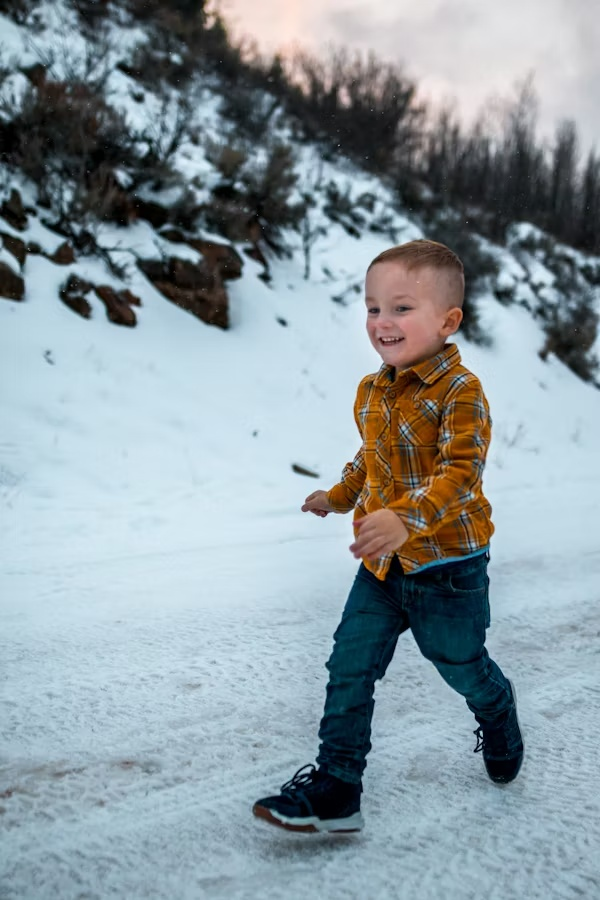
\includegraphics[width=0.72\textwidth, height=4.2cm, keepaspectratio]{SlideImages/happy_1.jpg}
\end{center}

\vspace{0.01cm}
\begin{exampleblock}{\normalsize \textbf{Base Caption}}
    \small \centering ``A young boy in a yellow jacket and blue jeans walks in the snow.''
\end{exampleblock}
\begin{alertblock}{\normalsize \textbf{Emotion-Aware Caption} \hfill \textcolor{yellow!50!orange}{Detected: Happy}}
    \small \centering ``A \textbf{happy} young boy in a yellow jacket and blue jeans walks in the snow.''
\end{alertblock}

\end{frame}

%% ═══════════════════════════════════════════════════════════════════
%% SLIDE 13 — Qualitative: Sad
%% ═══════════════════════════════════════════════════════════════════
\begin{frame}{Emotion-Aware Caption Example — \textcolor{yellow!50!orange}{\textbf{Sad}}}

\begin{center}
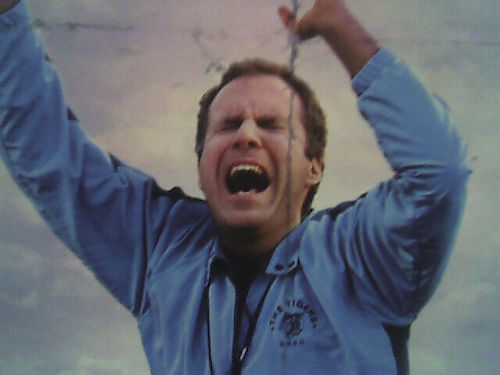
\includegraphics[width=0.72\textwidth, height=4.2cm, keepaspectratio]{SlideImages/sad_1.jpg}
\end{center}


\begin{exampleblock}{\normalsize \textbf{Base Caption}}
    \small \centering ``A young man with dark hair and a blue shirt is raising his hand up in the air''
\end{exampleblock}
\begin{alertblock}{\normalsize \textbf{Emotion-Aware Caption} \hfill \textcolor{yellow!50!orange}{Detected: Sad}}
    \small \centering ``A young \textbf{melancholic} man with dark hair and a blue shirt is raising his hand up in the air.''
\end{alertblock}

\end{frame}

%% ═══════════════════════════════════════════════════════════════════
%% SLIDE 14 — Qualitative: Angry
%% ═══════════════════════════════════════════════════════════════════
\begin{frame}{Emotion-Aware Caption Example — \textcolor{yellow!50!orange}{\textbf{Angry}}}

\begin{center}
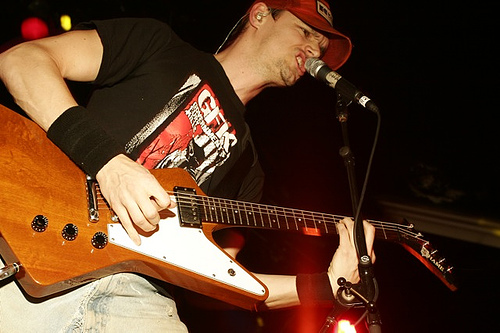
\includegraphics[width=0.72\textwidth, height=4.2cm, keepaspectratio]{SlideImages/angry_1.jpg}
\end{center}

\vspace{0.01cm}
\begin{exampleblock}{\normalsize \textbf{Base Caption}}
    \small \centering ``A  man in a red shirt is playing guitar and singing into a microphone''
\end{exampleblock}
\begin{alertblock}{\normalsize \textbf{Emotion-Aware Caption} \hfill \textcolor{yellow!50!orange}{Detected: Angry}}
    \small \centering ``An \textbf{angry} man in a red shirt is playing guitar and singing into a microphone.''
\end{alertblock}

\end{frame}

%% ═══════════════════════════════════════════════════════════════════
%% SLIDE 15 — Qualitative: Surprise
%% ═══════════════════════════════════════════════════════════════════
\begin{frame}{Emotion-Aware Caption Example — \textcolor{yellow!50!orange}{\textbf{Surprise}}}

\begin{center}
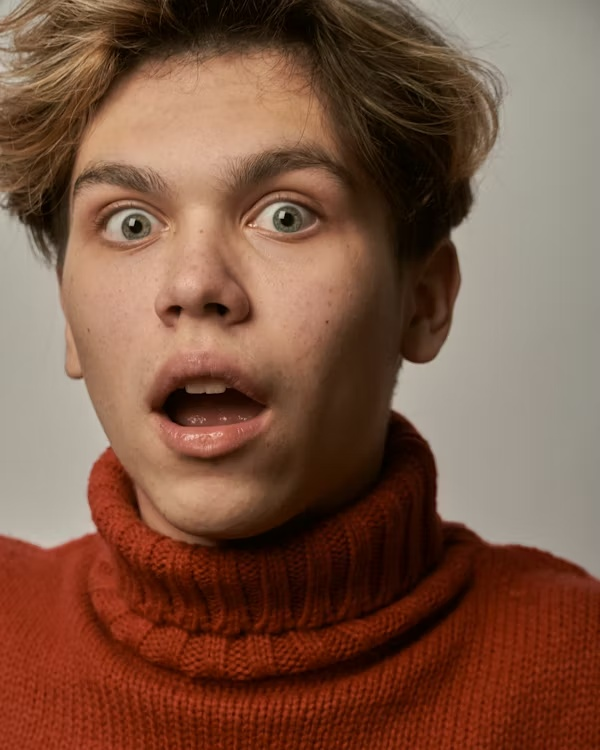
\includegraphics[width=0.72\textwidth, height=4.2cm, keepaspectratio]{SlideImages/surprise_1.jpg}
\end{center}

\vspace{0.01cm}
\begin{exampleblock}{\normalsize \textbf{Base Caption}}
    \small \centering ``A young boy with brown eyes and a white shirt is looking at the camera.''
\end{exampleblock}
\begin{alertblock}{\normalsize \textbf{Emotion-Aware Caption} \hfill \textcolor{yellow!50!orange}{Detected: Surprise}}
    \small \centering ``A young \textbf{surprised} boy with brown eyes and a white shirt is looking at the camera.''
\end{alertblock}

\end{frame}

%% ═══════════════════════════════════════════════════════════════════
%% SLIDE 16 — Qualitative: Fear
%% ═══════════════════════════════════════════════════════════════════
\begin{frame}{Emotion-Aware Caption Example — \textcolor{yellow!50!orange}{\textbf{Fear}}}

\begin{center}
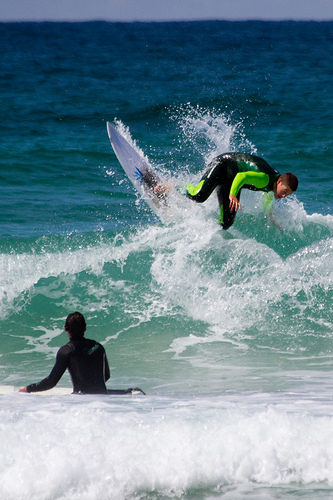
\includegraphics[width=0.72\textwidth, height=4.2cm, keepaspectratio]{SlideImages/fear_1.jpg}
\end{center}

\vspace{0.01cm}
\begin{exampleblock}{\normalsize \textbf{Base Caption}}
    \small \centering ``A surfer in a black wetsuit surfs in the ocean with a wave in the background.''
\end{exampleblock}
\begin{alertblock}{\normalsize \textbf{Emotion-Aware Caption} \hfill \textcolor{yellow!50!orange}{Detected: Fear}}
    \small \centering ``A \textbf{fearful} surfer in a black wetsuit surfs in the ocean with a wave in the background.''
\end{alertblock}

\end{frame}

%% ═══════════════════════════════════════════════════════════════════
%% SLIDE 17 — Qualitative: Disgust
%% ═══════════════════════════════════════════════════════════════════
\begin{frame}{Emotion-Aware Caption Example — \textcolor{yellow!50!orange}{\textbf{Disgust}}}

\begin{center}
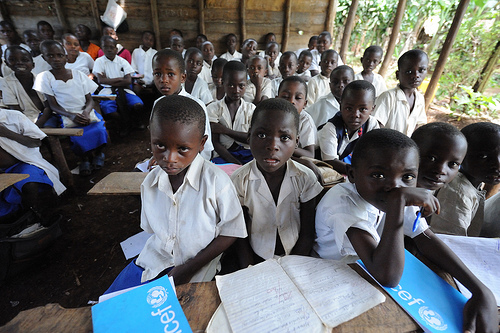
\includegraphics[width=0.72\textwidth, height=4.2cm, keepaspectratio]{SlideImages/disgust_1.jpg}
\end{center}

\vspace{0.01cm}
\begin{exampleblock}{\normalsize \textbf{Base Caption}}
    \small \centering ``A group of students are watching a conference performance in a fancy class.''
\end{exampleblock}
\begin{alertblock}{\normalsize \textbf{Emotion-Aware Caption} \hfill \textcolor{yellow!50!orange}{Detected: Disgust}}
    \small \centering ``A \textbf{disgusted} group of students are watching a conference performance in a fancy class.''
\end{alertblock}

\end{frame}

%% ═══════════════════════════════════════════════════════════════════
%% SLIDE 18 — Qualitative: Neutral
%% ═══════════════════════════════════════════════════════════════════
\begin{frame}{Emotion-Aware Caption Example — \textcolor{yellow!50!orange}{\textbf{Neutral}}}

\begin{center}
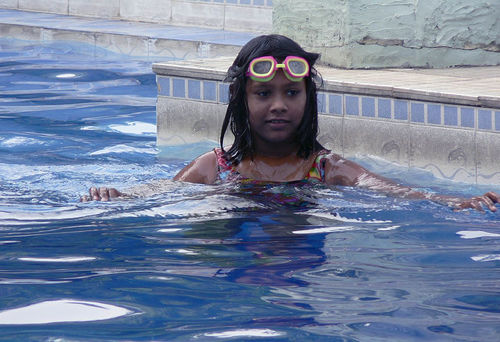
\includegraphics[width=0.72\textwidth, height=4.2cm, keepaspectratio]{SlideImages/neutral_1.jpg}
\end{center}

\vspace{0.01cm}
\begin{exampleblock}{\normalsize \textbf{Base Caption}}
    \small \centering ``A young girl with a swimsuit and goggles comes her head from above a pool.''
\end{exampleblock}
\begin{alertblock}{\normalsize \textbf{Emotion-Aware Caption} \hfill \textcolor{yellow!50!orange}{Detected: Neutral}}
    \small \centering ``A young \textbf{calm} girl with a swimsuit and goggles comes her head from above a pool.''
\end{alertblock}

\end{frame}

%% ═══════════════════════════════════════════════════════════════════
%% SLIDE 19 — Live Demo: Vercel Screenshot 1 (Happy)
%% ═══════════════════════════════════════════════════════════════════
\begin{frame}{Live Web App — Demo Screenshot (Happy)}

\begin{center}
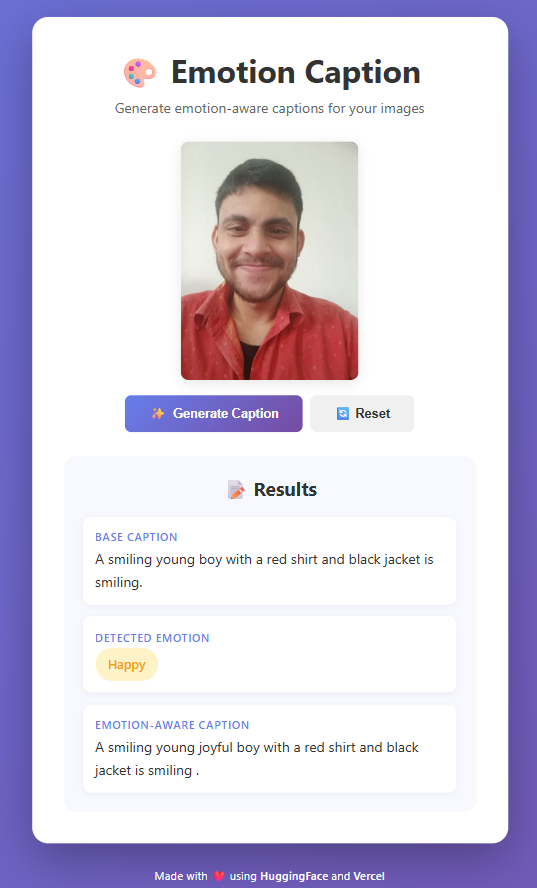
\includegraphics[width=\textwidth, height=0.82\textheight, keepaspectratio]{SlideImages/anuron_happy.png}
\end{center}

\end{frame}

%% ═══════════════════════════════════════════════════════════════════
%% SLIDE 20 — Live Demo: Vercel Screenshot 2 (Angry)
%% ═══════════════════════════════════════════════════════════════════
\begin{frame}{Live Web App — Demo Screenshot (Angry)}

\begin{center}
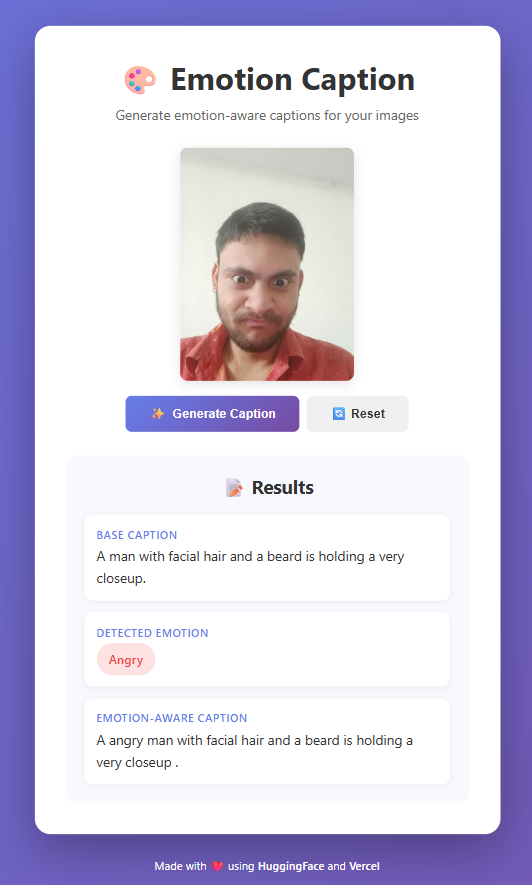
\includegraphics[width=\textwidth, height=0.82\textheight, keepaspectratio]{SlideImages/anuron_angry.png}
\end{center}

\end{frame}


%% ═══════════════════════════════════════════════════════════════════
%% SLIDE 14 — Deployment
%% ═══════════════════════════════════════════════════════════════════
\begin{frame}{Deployment Architecture}

    \begin{columns}[T]
    \begin{column}{0.50\textwidth}
        \textbf{Backend:}
        \begin{itemize}
            \item \textbf{FastAPI} (Python) on HuggingFace Spaces
            \item Docker container (Python 3.10-slim)
            \item Model downloaded from HuggingFace Hub on startup
            \item Endpoints: \texttt{GET /} (health check), \texttt{POST /api/caption}
            \item \textbf{URL:}\\
                  \tiny\url{https://HimadriBiswas-emotion-caption-api.hf.space}
        \end{itemize}
    \end{column}
    \begin{column}{0.48\textwidth}
        \textbf{Frontend:}
        \begin{itemize}
            \item \textbf{React 18} on Vercel
            \item Drag-and-drop image upload
            \item Displays: base caption, emotion badge, emotion-aware caption
            \item \textbf{URL:}\\
                  \tiny\url{https://emotion-caption-frontend.vercel.app}
        \end{itemize}
    \end{column}
    \end{columns}

    \vspace{0.4cm}
    \textbf{Deployment Challenges Solved:}
    \begin{itemize}
        \item Model (1.91~GB) $>$ HuggingFace 1~GB limit $\to$ stored separately in HF Models Hub
        \item TensorFlow 2.13.0 compatibility pinned for DeepFace
        \item Replaced \texttt{libgl1-mesa-glx} with \texttt{libgl1} in Dockerfile
    \end{itemize}

    \vspace{0.2cm}
    \begin{block}{Total Cost}
        \centering \$0/month — fully free-tier deployment
    \end{block}

\end{frame}

%% ═══════════════════════════════════════════════════════════════════
%% SLIDE 15 — Limitations & Future Work
%% ═══════════════════════════════════════════════════════════════════
\begin{frame}{Limitations \& Future Work}

    \textbf{Current Limitations:}
    \begin{itemize}
        \item Adjective insertion can be grammatically awkward (e.g., plural nouns)
        \item Only dominant emotion from most prominent face is used
        \item Semantic mismatch: ``disgusted person'' vs.\ the intended meaning
        \item Little gibberish base captions on completely new images
    \end{itemize}

    \vspace{0.4cm}
    \textbf{Future Directions:}
    \begin{itemize}
        \item \textbf{Multiple face} emotion handling per image
        \item \textbf{Semantic validators} for more natural adjective choice
        \item \textbf{Model quantization} to reduce size and cold-start time
        \item \textbf{Video captioning} with temporal emotion tracking
    \end{itemize}

\end{frame}

%% ═══════════════════════════════════════════════════════════════════
%% SLIDE 16 — References  (NEW — placed before Conclusion)
%% ═══════════════════════════════════════════════════════════════════
\begin{frame}{References}

    \begin{enumerate}\small
        \item Mishra, S.\ et al., \textit{Image Caption Generation using Vision Transformer and GPT Architecture}. 2024 2nd International Conference on Advancement in Computation \& Computer Technologies (InCACCT). DOI: \url{https://doi.org/10.1109/InCACCT61598.2024.10551257}

        \vspace{0.55cm}
        \item Venkatesan, R.; Shirly, S.; Selvarathi, M.; Jebaseeli, T.J., \textit{Human Emotion Detection Using DeepFace and Artificial Intelligence}. \textit{Engineering Proceedings} 2023, 59(37). DOI: \url{https://doi.org/10.3390/engproc2023059037}
    \end{enumerate}

\end{frame}

%% ═══════════════════════════════════════════════════════════════════
%% SLIDE 17 — Conclusion
%% ═══════════════════════════════════════════════════════════════════
\begin{frame}{Conclusion}

    \begin{block}{Summary of Achievements}
        \begin{itemize}
            \item Built a complete \textbf{3-stage emotion-aware image captioning pipeline}
            \item Achieved \textbf{METEOR 44.18\%} on Flickr30k dataset
            \item Successfully integrated \textbf{7-category emotion detection} via DeepFace
            \item Deployed as a \textbf{live web application} at zero cost
            \item Full open codebase on Kaggle Notebook
        \end{itemize}
    \end{block}

    \vspace{0.5cm}
    \textbf{Key Takeaway:}\\[0.3em]
    Combining pre-trained ViT + GPT-2 with rule-based emotion integration provides
    a pragmatic, lightweight approach to \textbf{emotionally-aware image descriptions}.\\[0.4em]
    This bridges the gap between \textit{what} machines see and \textit{how} humans feel.

\end{frame}

%% ═══════════════════════════════════════════════════════════════════
%% SLIDE 18 — Thank You
%% ═══════════════════════════════════════════════════════════════════
\begin{frame}
    \centering
    \vspace{1cm}
    {\Huge \textbf{Thank You!}}\\[1cm]
    \begin{tabular}{rl}
    \textbf{Live Demo:} & \url{https://emotion-caption-frontend.vercel.app} \\[0.4em]
    \textbf{Team:}      & TeamML Newbies \\
    \end{tabular}
\end{frame}

%%%%%%%%%%%%%%%%%%%%%%%%%%%%%%%%%%%%%%%%%%%%%%%%%%%%%%%%%%%%%%%%%%%%
\end{document}
%%%%%%%%%%%%%%%%%%%%%%%%%%%%%%%%%%%%%%%%%%%%%%%%%%%%%%%%%%%%%%%%%%%%